%!TEX root = ../thesis.tex
%*******************************************************************************
%***************************** Fifth Chapter **********************************
%*******************************************************************************
\graphicspath{{Chapter5/Figs/Vector/}{Chapter5/Figs/}}

%%%%%%%%%%%%%%%%%%%%%%%%%%%%%%%%%%%%%%%%%%%%%%%%%%%%%%%%%%%%%%%%%%%%%%%%%%%%%%%%
% The Portal
%%%%%%%%%%%%%%%%%%%%%%%%%%%%%%%%%%%%%%%%%%%%%%%%%%%%%%%%%%%%%%%%%%%%%%%%%%%%%%%%
% - Is it possible to communicate the inner workings of the system through the
%   user interface?
% #region
\chapter{The Portal}
\section{Introduction}
The term 'reasoning' in the title, meaning "the action of thinking about something in a logical, sensible way", may have been redundant if a system were to calculate trip prices autonomously --- this system is designed with the user in mind. That is why the inner workings of the system must be expressed in such a way that given some rule as input, the user will be able to logically derive the consequential output with confidence.
% #endregion

%%%%%%%%%%%%%%%%%%%%%%%%%%%%%%%%%%%%%%%%%%%%%%%%%%%%%%%%%%%%%%%%%%%%%%%%%%%%%%%%
% Visual Hierarchy
%%%%%%%%%%%%%%%%%%%%%%%%%%%%%%%%%%%%%%%%%%%%%%%%%%%%%%%%%%%%%%%%%%%%%%%%%%%%%%%%
% #region
\section{Design}
A pricing rule is nothing more than a set of prices and collection of criteria by which a trip must abide in order for those prices to apply. These criteria and pricing information are stored in database entities, which could be expressed as components in a view. For example, "the pickup location of a trip must be located in Amsterdam" is a criterion that is stored in a location entity, that may be expressed as polygon on a world map component. Even if the possible combinations of criteria could be graphed, it would be highly dimensional.

\subsection{Essential Components}
The main entities that make up a the price calculation system are visualized in Figure \ref{fig:Treemap}. The plurality of the child entities describe whether more than one child are present within the parent entity. For example, rules have many products, with each product having one price, which has one priceFixed and one priceDynamic.

\begin{figure}[H]
	\centering
	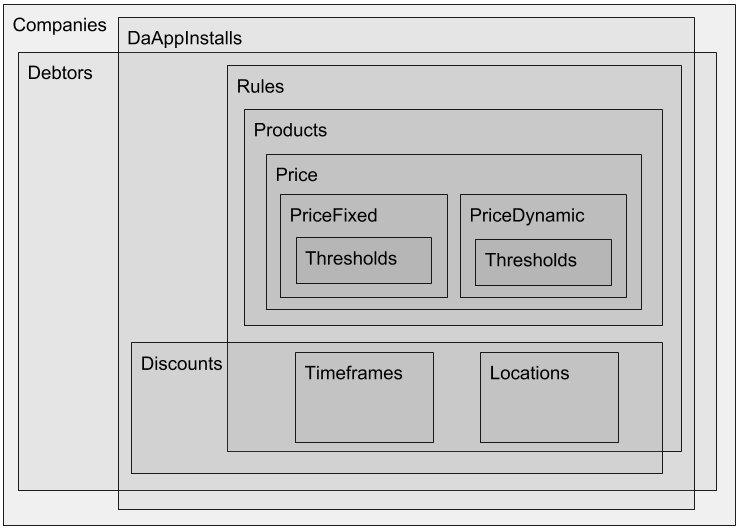
\includegraphics[width=0.9\textwidth]{Treemap}
	\caption[Treemap of Components]{Treemap of components.}
	\label{fig:Treemap}
\end{figure}

\subsection{Expressing Order}
Figure \ref{fig:Treemap} taps into the ability of the reader to preattentively process the images structure. It is immediately evident that Discounts have a subset of the entities that Rules have, and that Debtors and DaAppInstalls have the same entity relationships. The brain has already ordered the differently sized boxes by enclosure, proximity, intensity, and spatial grouping. Stephen Few states that "Perception of these basic visual attributes is called 'preattentive' processing, in contrast to the conscious part of perception, which is called 'attentive' processing. Preattentive processing is extremely fast and broadband in that we can simultaneously perceive a large number of these basic visual attributes, called 'preattentive attributes'. Preattentive perception is done in parallel, but attentive processing is done serially and is, therefore, much slower." in \cite[p.~3]{few}. This fact can be utilized to construct a hierarchy through visual queues. A famous phrase often used in data visualizations called Shneiderman's mantra \cite{mantra}, lays the foundation of principles that enable a user to maintain an understanding of the context in which data is visualized. The sentences in the mantra dictate that there are three stages in data exploration.

\begin{enumerate}
	\item Overview First
	\item Zoom and Filter
	\item Details on Demand
\end{enumerate}

Pricing rules cannot be plotted in a graph, yet this mantra in combination with preattentive attributes could be put to good use in reducing the cognitive overhead while reasoning about pricing rules.
% #endregion

%%%%%%%%%%%%%%%%%%%%%%%%%%%%%%%%%%%%%%%%%%%%%%%%%%%%%%%%%%%%%%%%%%%%%%%%%%%%%%%%
% Design
%%%%%%%%%%%%%%%%%%%%%%%%%%%%%%%%%%%%%%%%%%%%%%%%%%%%%%%%%%%%%%%%%%%%%%%%%%%%%%%%
% #region
\section{Visual Hierarchy}
In order to communicate the criteria of one pricing rule, the system must guide the user from an overview down to the less important details of the rule. This is to be achieved by splitting up the various criteria into multiple views. What this means is that the user is limited to only reason about a subset of the criteria at once. For example, the user is obligated to first define a location, before it is assigned to a rule, splitting problems into smaller portions. The mantra could be translated into the design on multiple levels. Some components are easy to reason about, and could be combined with other components to make up one view. For example, one rule can have many product entities, and each product has a price entity. These components could compose a single view, having one rule and a list of products with their respective prices. The existing pages in the portal already follow a basic hierarchy:

\begin{enumerate}
	\item Overview: enumerates over a list of entities
	\item Detail page: contains one particular entity
	\item Composite page: displays a combination of lists of entities and/or single entities that belong together
\end{enumerate}

Entities that are part of a many-to-many or one-to-many relation should have their own overview and detail pages, otherwise the user may think that a particular entity that is combined into another entity's view, may exist for that entity only. If the user modifies that entity, it has consequences for all other relationships with that entity. For example, if a location was shared between many rules, the user could edit the address of the location, unaware of the consequences that the change brings to all the rules that depend on that particular location. One-to-one or many-to-one relationships do not have that problem. For example, thresholds are embedded, meaning that they are not part of any entity other than the one that embeds them. With this concept, the following entities should have their own overview and detail pages: Products, Locations, Rules, Discounts, and DaAppInstalls. The mantra could also be applied to the representation of entity properties in the same fashion. But for each enumeration, a direction of space on the page must be filled. As a webpage only has two dimensions of space, the properties that fill up the space must be grouped in some fashion. Preattentive attributes can be utilized to illustrate that some elements on composite pages belong to each other, or are in fact distinct.
% #endregion

%%%%%%%%%%%%%%%%%%%%%%%%%%%%%%%%%%%%%%%%%%%%%%%%%%%%%%%%%%%%%%%%%%%%%%%%%%%%%%%%
% Products
%%%%%%%%%%%%%%%%%%%%%%%%%%%%%%%%%%%%%%%%%%%%%%%%%%%%%%%%%%%%%%%%%%%%%%%%%%%%%%%%
% #region
\section{Products}
Users are allowed to view the list of products that have been created. Products can be selected, upon which the user is taken to the detail page where the type, name and other properties can be set, and where the product may be deleted. When a property has changed, the save button becomes available. And when the user tries to leave the page after changing a property, a prompt is shown that allows the user to leave or continue editing a product.

\begin{figure}[H]
	\centering
	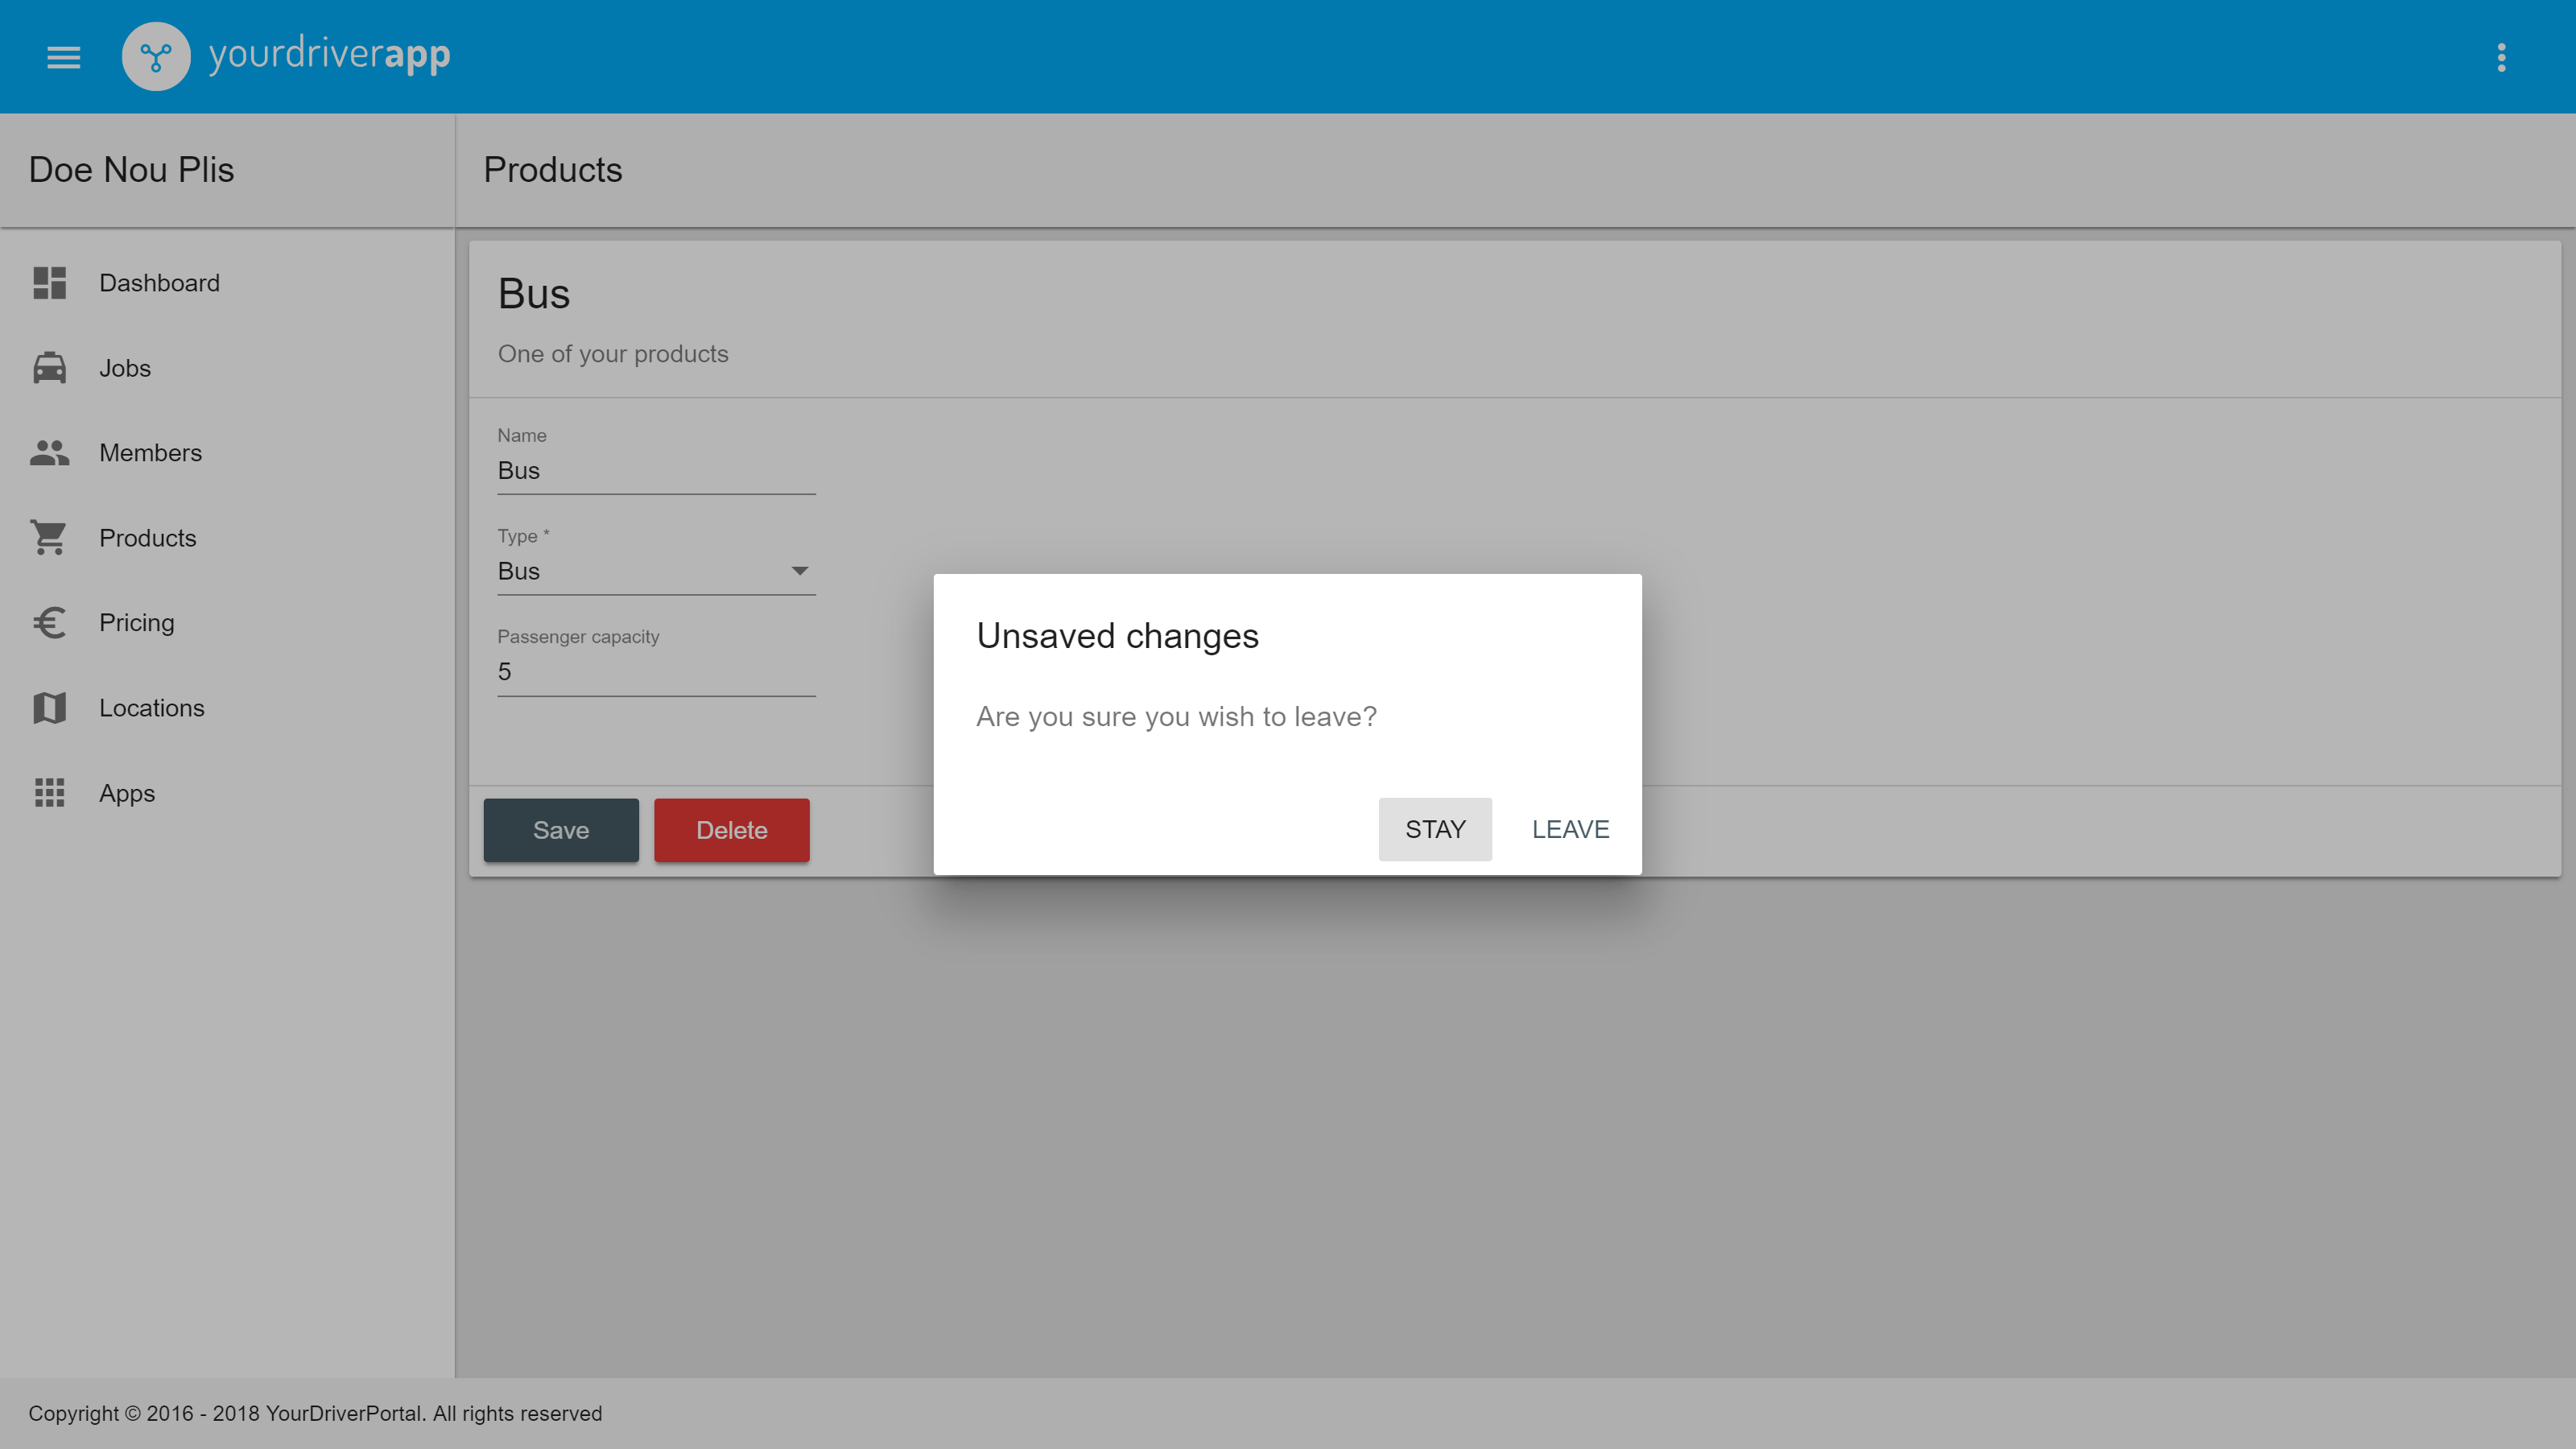
\includegraphics[width=0.9\textwidth]{Products}
	\caption[Products Component]{Products with a warning prompt.}
	\label{fig:Products Component}
\end{figure}

These features have been implemented in every detail page for consistency, and have been shown in Figure \ref{fig:Products Component} because the product detail page itself is simple enough to allow a distraction.
% #endregion

%%%%%%%%%%%%%%%%%%%%%%%%%%%%%%%%%%%%%%%%%%%%%%%%%%%%%%%%%%%%%%%%%%%%%%%%%%%%%%%%
% Pricing
%%%%%%%%%%%%%%%%%%%%%%%%%%%%%%%%%%%%%%%%%%%%%%%%%%%%%%%%%%%%%%%%%%%%%%%%%%%%%%%%
% #region
\section{Pricing}
When the user navigates to the pricing view, a table with two tabs, 'rules' and 'special rates', is displayed. The special rates refer to discounts, but that word would imply that these records would only be able to make trips cheaper. Special rates can be negative or positive, and can be expressed in percentages and fixed amounts. For the sake of consistency, special rates will be referred to as discounts. Discounts and Rules have a lot in common, both allowing criteria to be applied through timeframes and locations. They can both be prioritized and they are the only entities that have an impact on trip prices.

\subsection{Discounts}
On the discount detail page, the name, priority, type and value properties may be set. When the type is changed between 'fixed' and 'percentage', the symbol next to the value changes from a \euro to a \% symbol. The timeframes and locations can be found underneath the normal properties. For the timeframes a component has been created that can be integrated into any page that requires a timeframe selector. Timeframes consist of two dates between which a discount or rule is active. A date picker allows users specify the date, while a separate time input allows users to specify the time. When users want to define more complex timeframes, a specific week days option opens up an hour selection element. When this option is enabled, the time inputs are hidden. They are mutually exclusive to avoid confusion between the time aspect of the timeframes.

%###############################################################################
% TIMEFRAME PICKER SCREENSHOT
%###############################################################################
\begin{figure}[H]
	\centering
	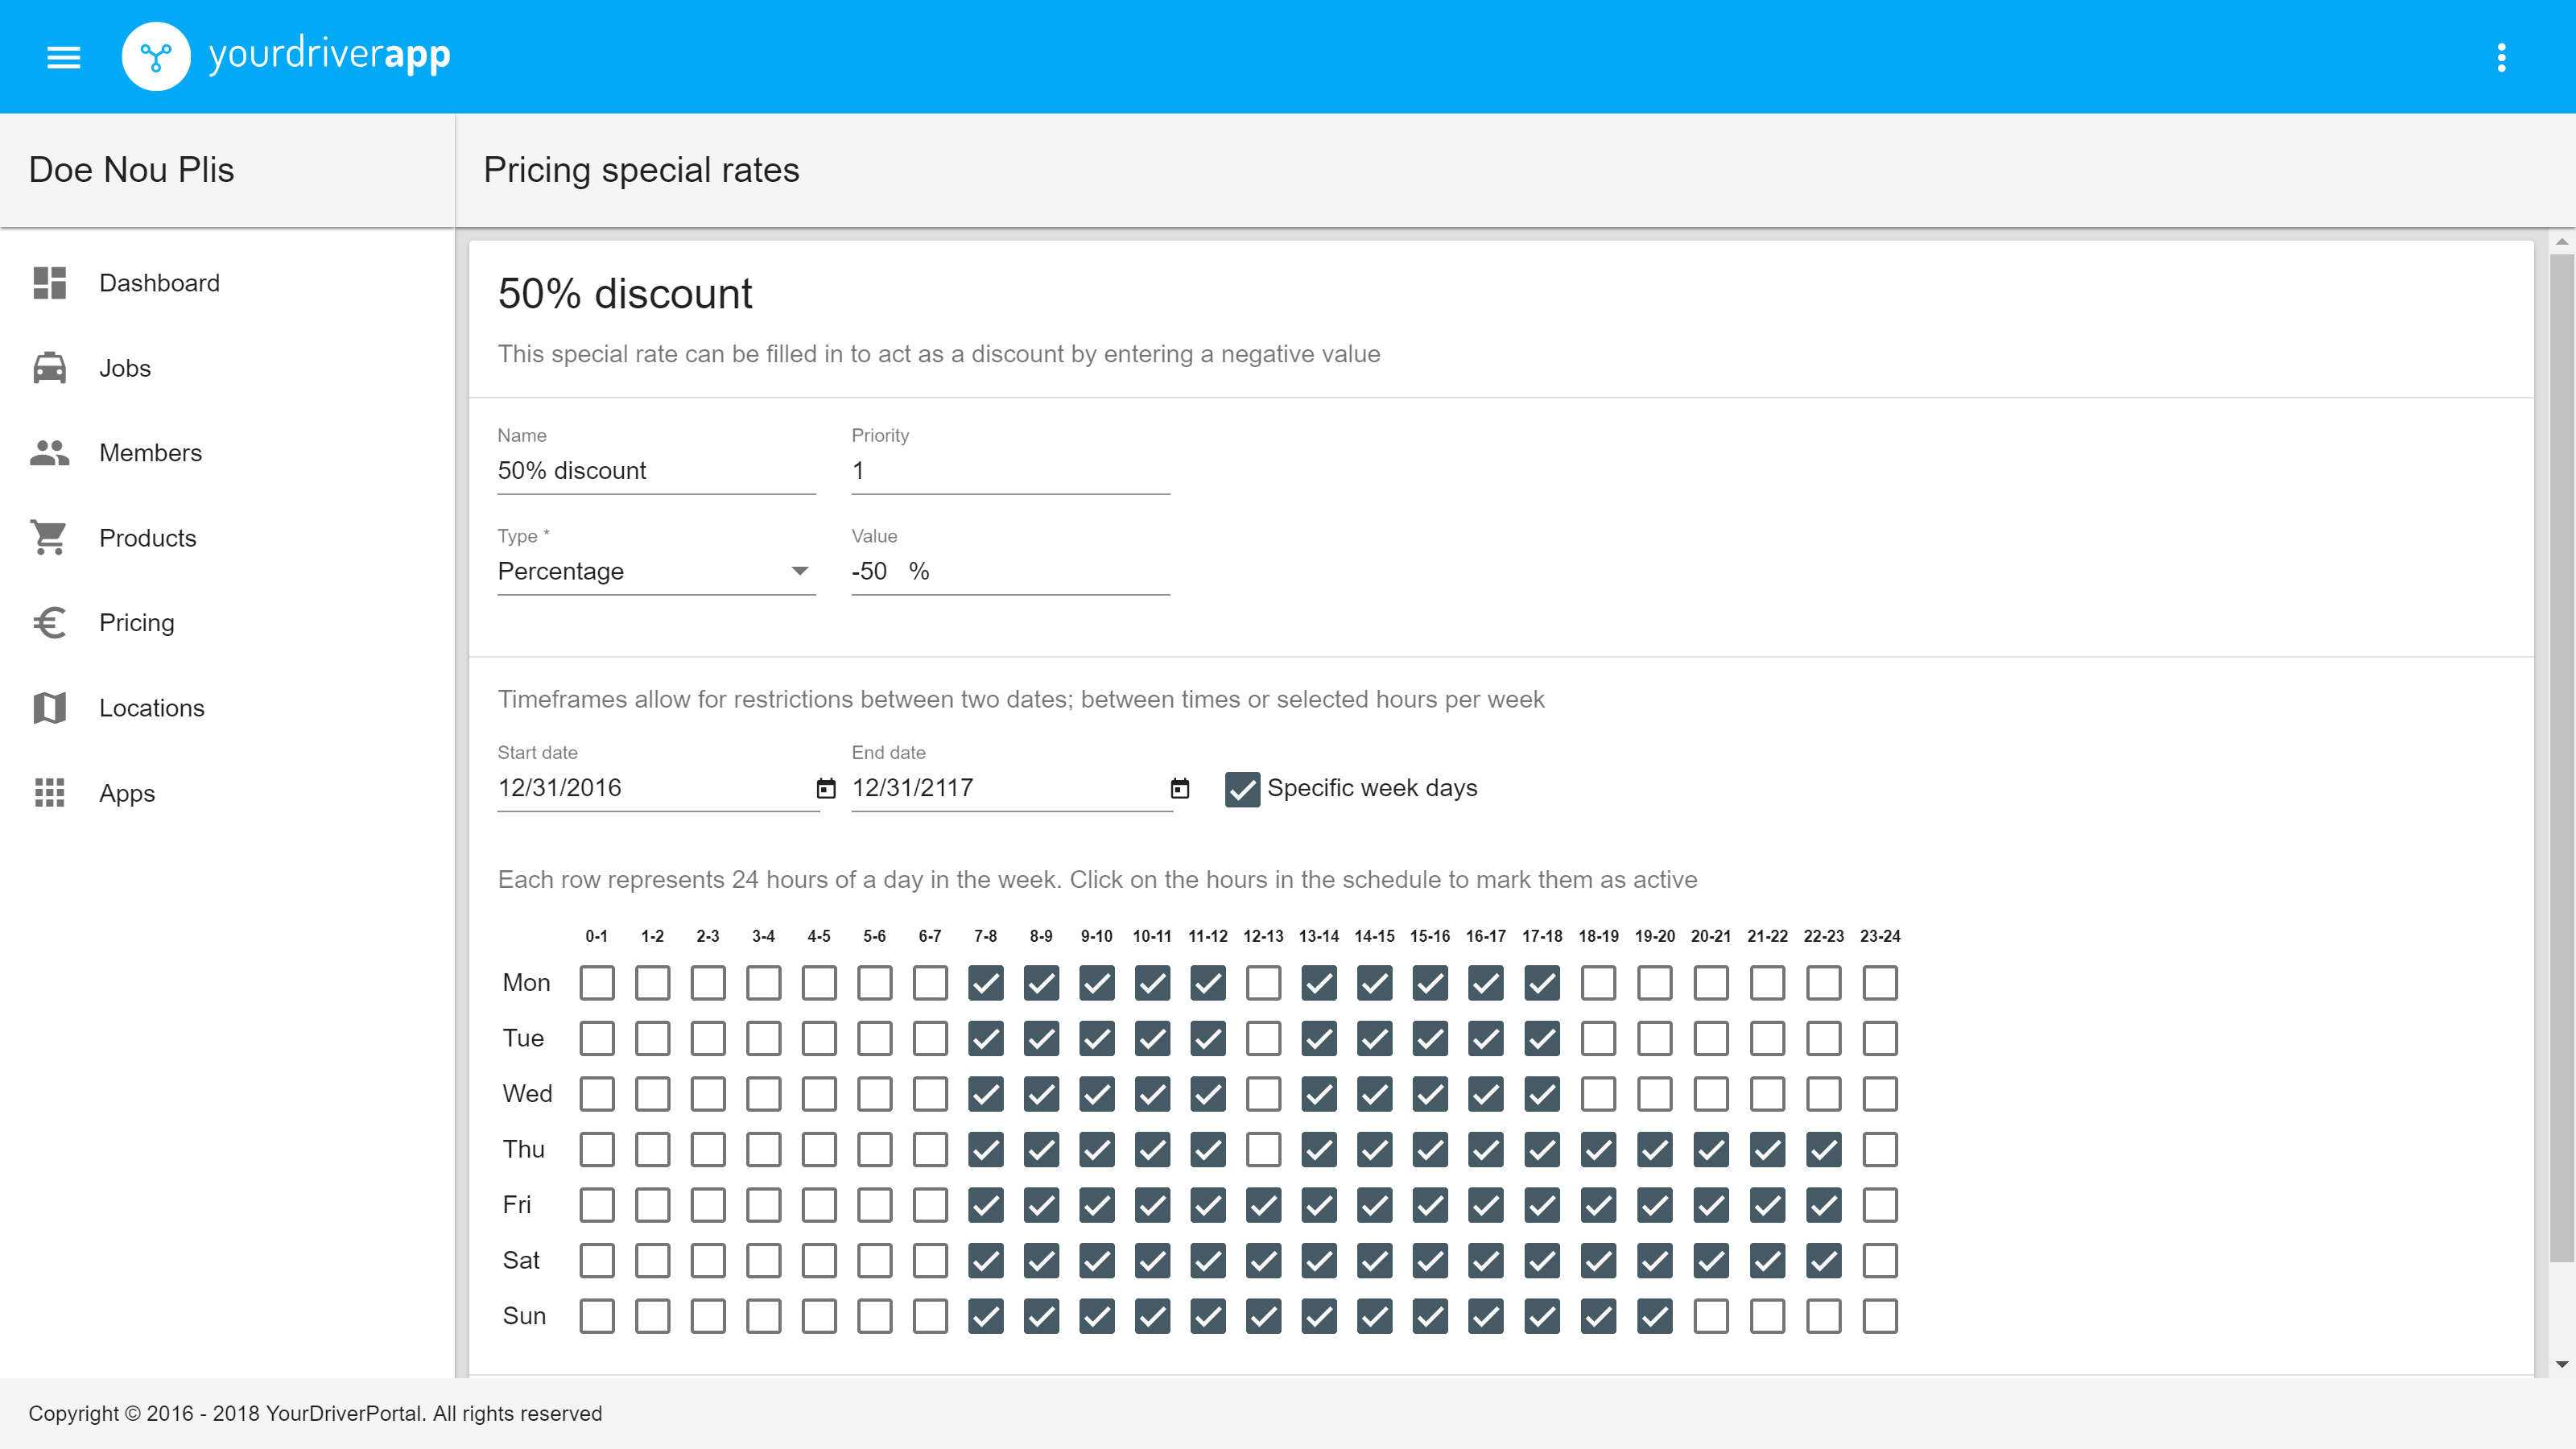
\includegraphics[width=0.9\textwidth]{Timeframes}
	\caption[Timeframe Component]{Timeframe with specific week days selector unfolded.}
	\label{fig:Timeframe Selector}
\end{figure}

When this toggle is set, the time aspect of the start and end date is hidden, as from that moment, time can only be defined as individual hours. Because this aspect of the timeframe is stored as a bit string, it is easily translated into an html input element, and can easily be modified in the future. Right above the timeframe selector component sits the location selector component. It has a 'from' and a 'to' input in which the user may enter a location by name or address. Autocompletion displays search results underneath the inputs allowing the user to quickly find a predefined location. When the user presses enter and the location does not exist, the user is prompted to create a new location. All locations that have been created by developers can be shared. This is added as a requirement in a later stage that allows users to create pricing rules right away, without having to bother with locations first.

%###############################################################################
% LOCATION PICKER SCREENSHOT
%###############################################################################
\begin{figure}[H]
	\centering
	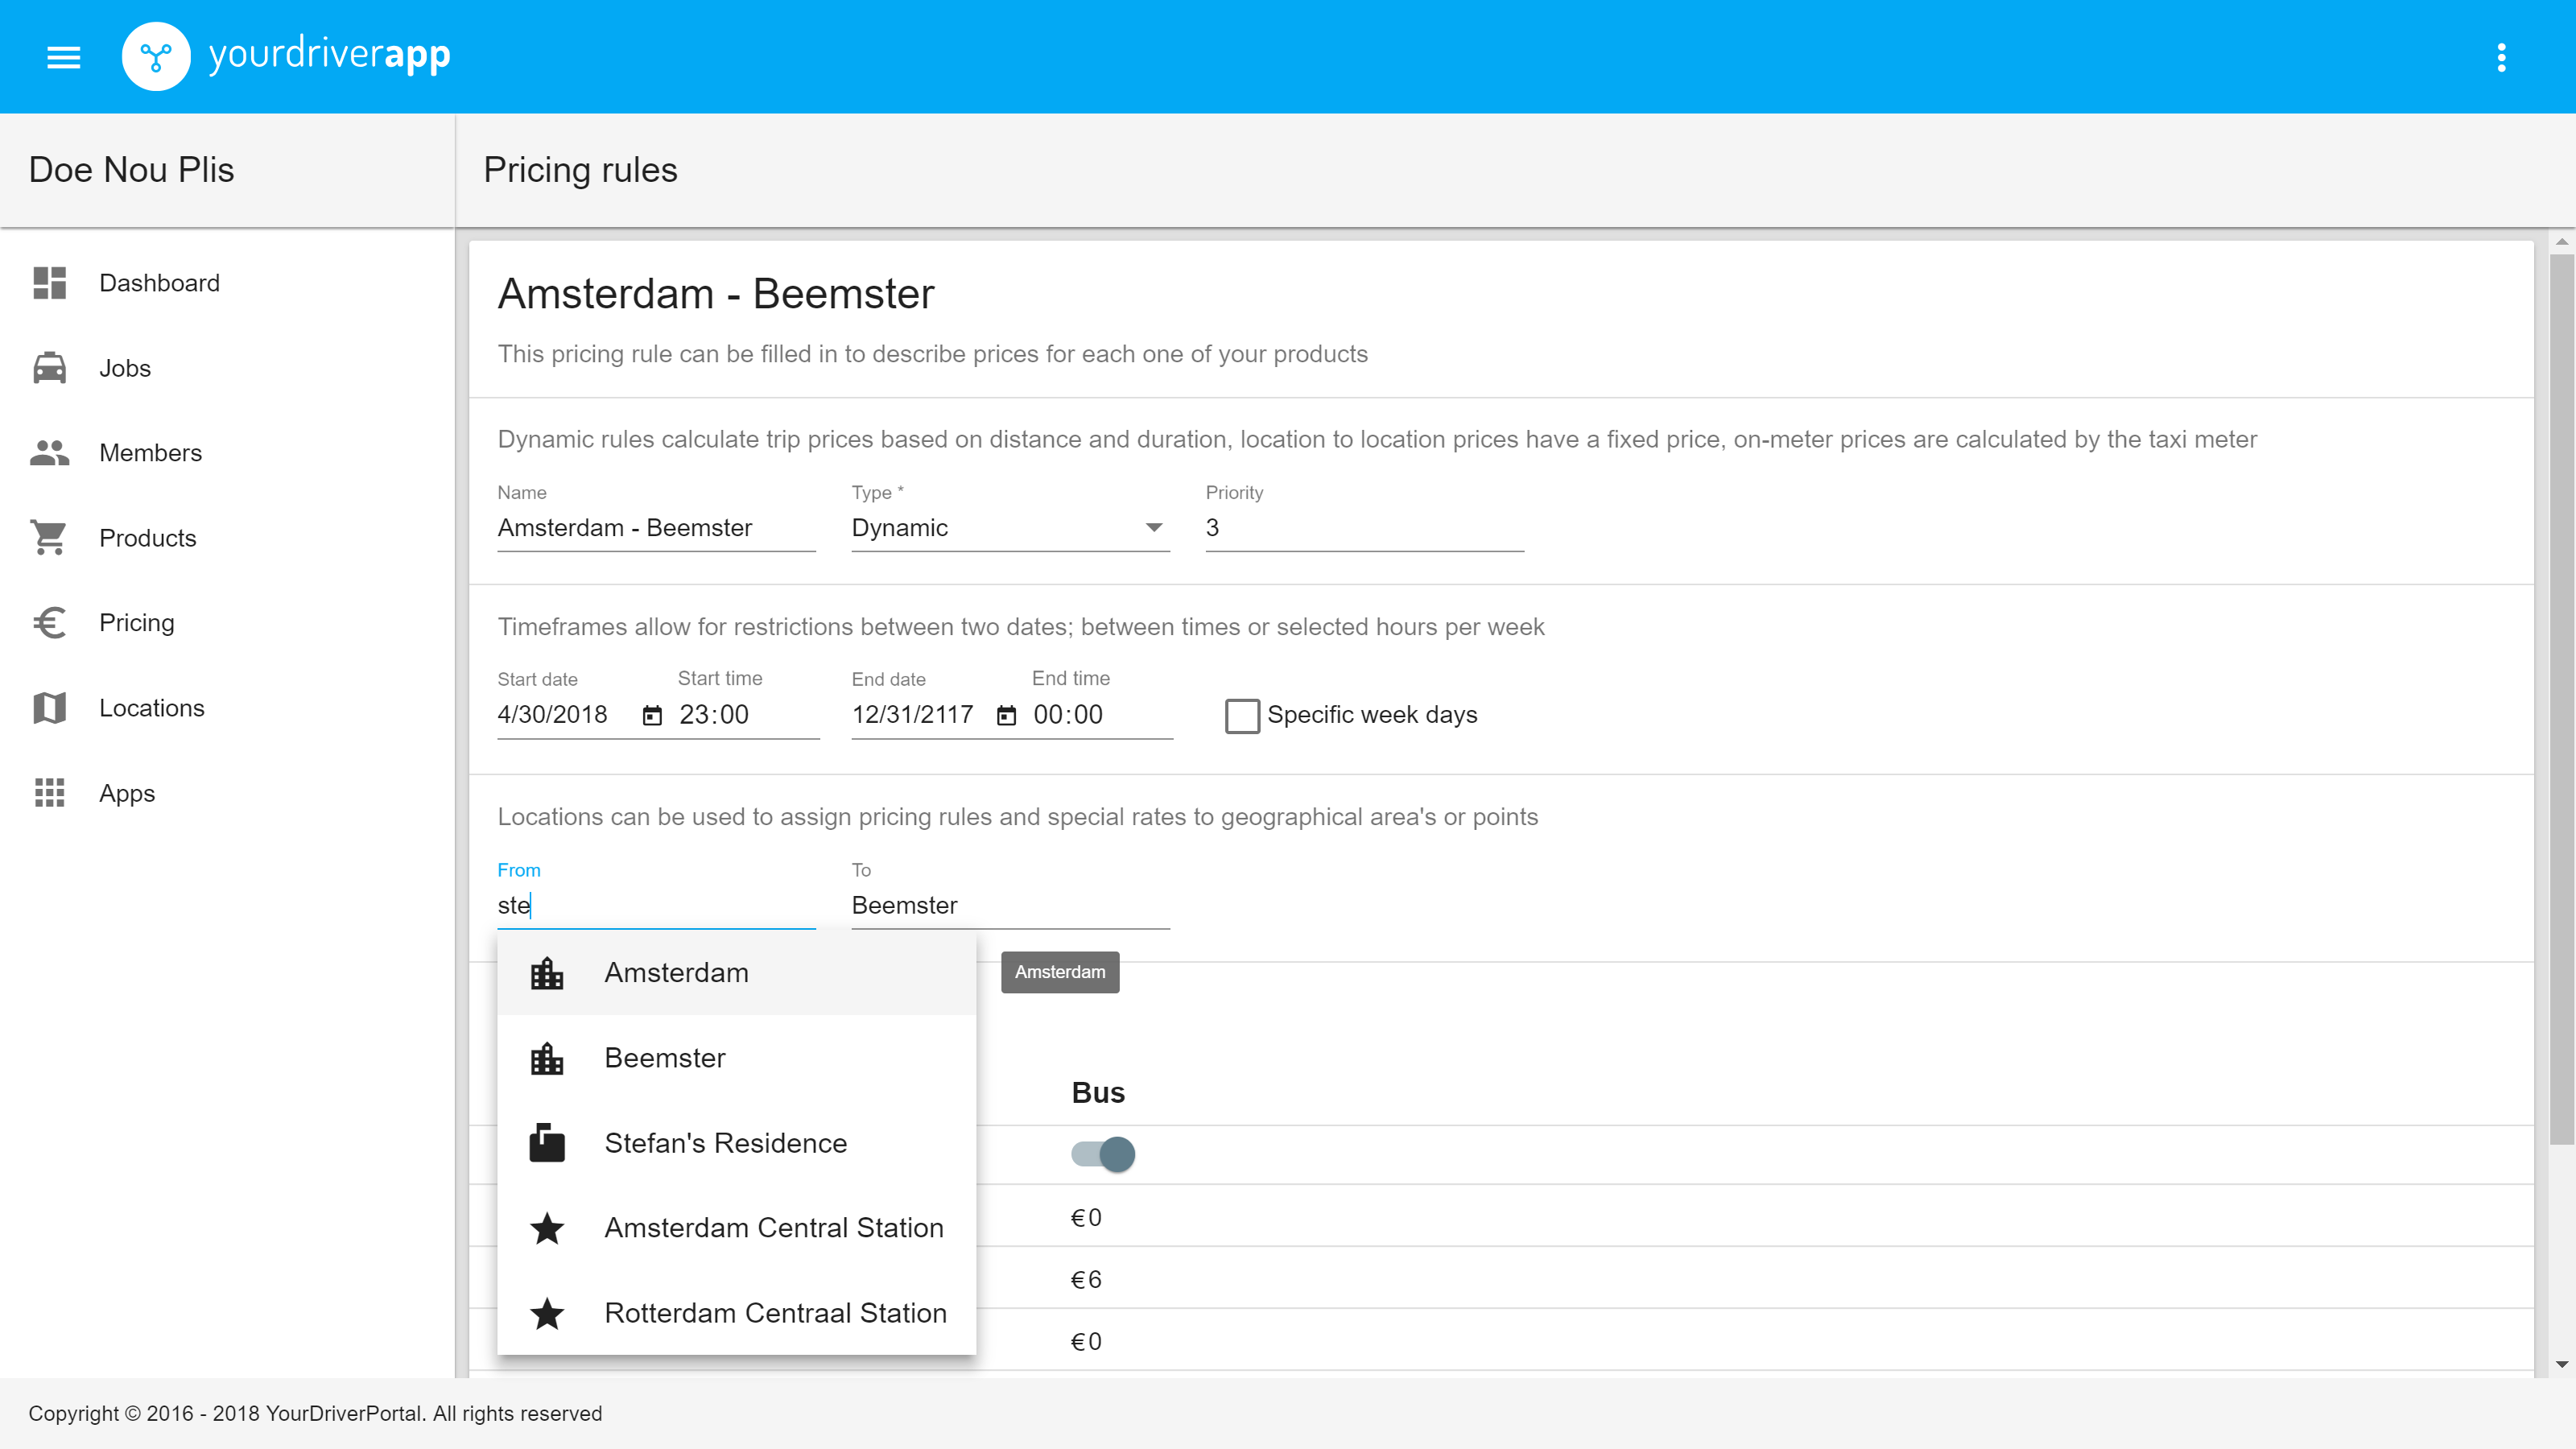
\includegraphics[width=0.9\textwidth]{Rules}
	\caption[Rules Component]{Location picker.}
	\label{fig:Location Selector}
\end{figure}

When the input is empty, the 'Everywhere' option is shown, which ensures that no location is associated with that input.

\subsection{Rules}
On top of the functionalities just covered, the rule detail page has more complex property inputs. A table of columns for each product is displayed in which the minimum price, waiting price, start price, kilometer price, and minute price inputs can be found on each row.

%###############################################################################
% DYNAMIC FORM SCREENSHOT
%###############################################################################
\begin{figure}[H]
	\centering
	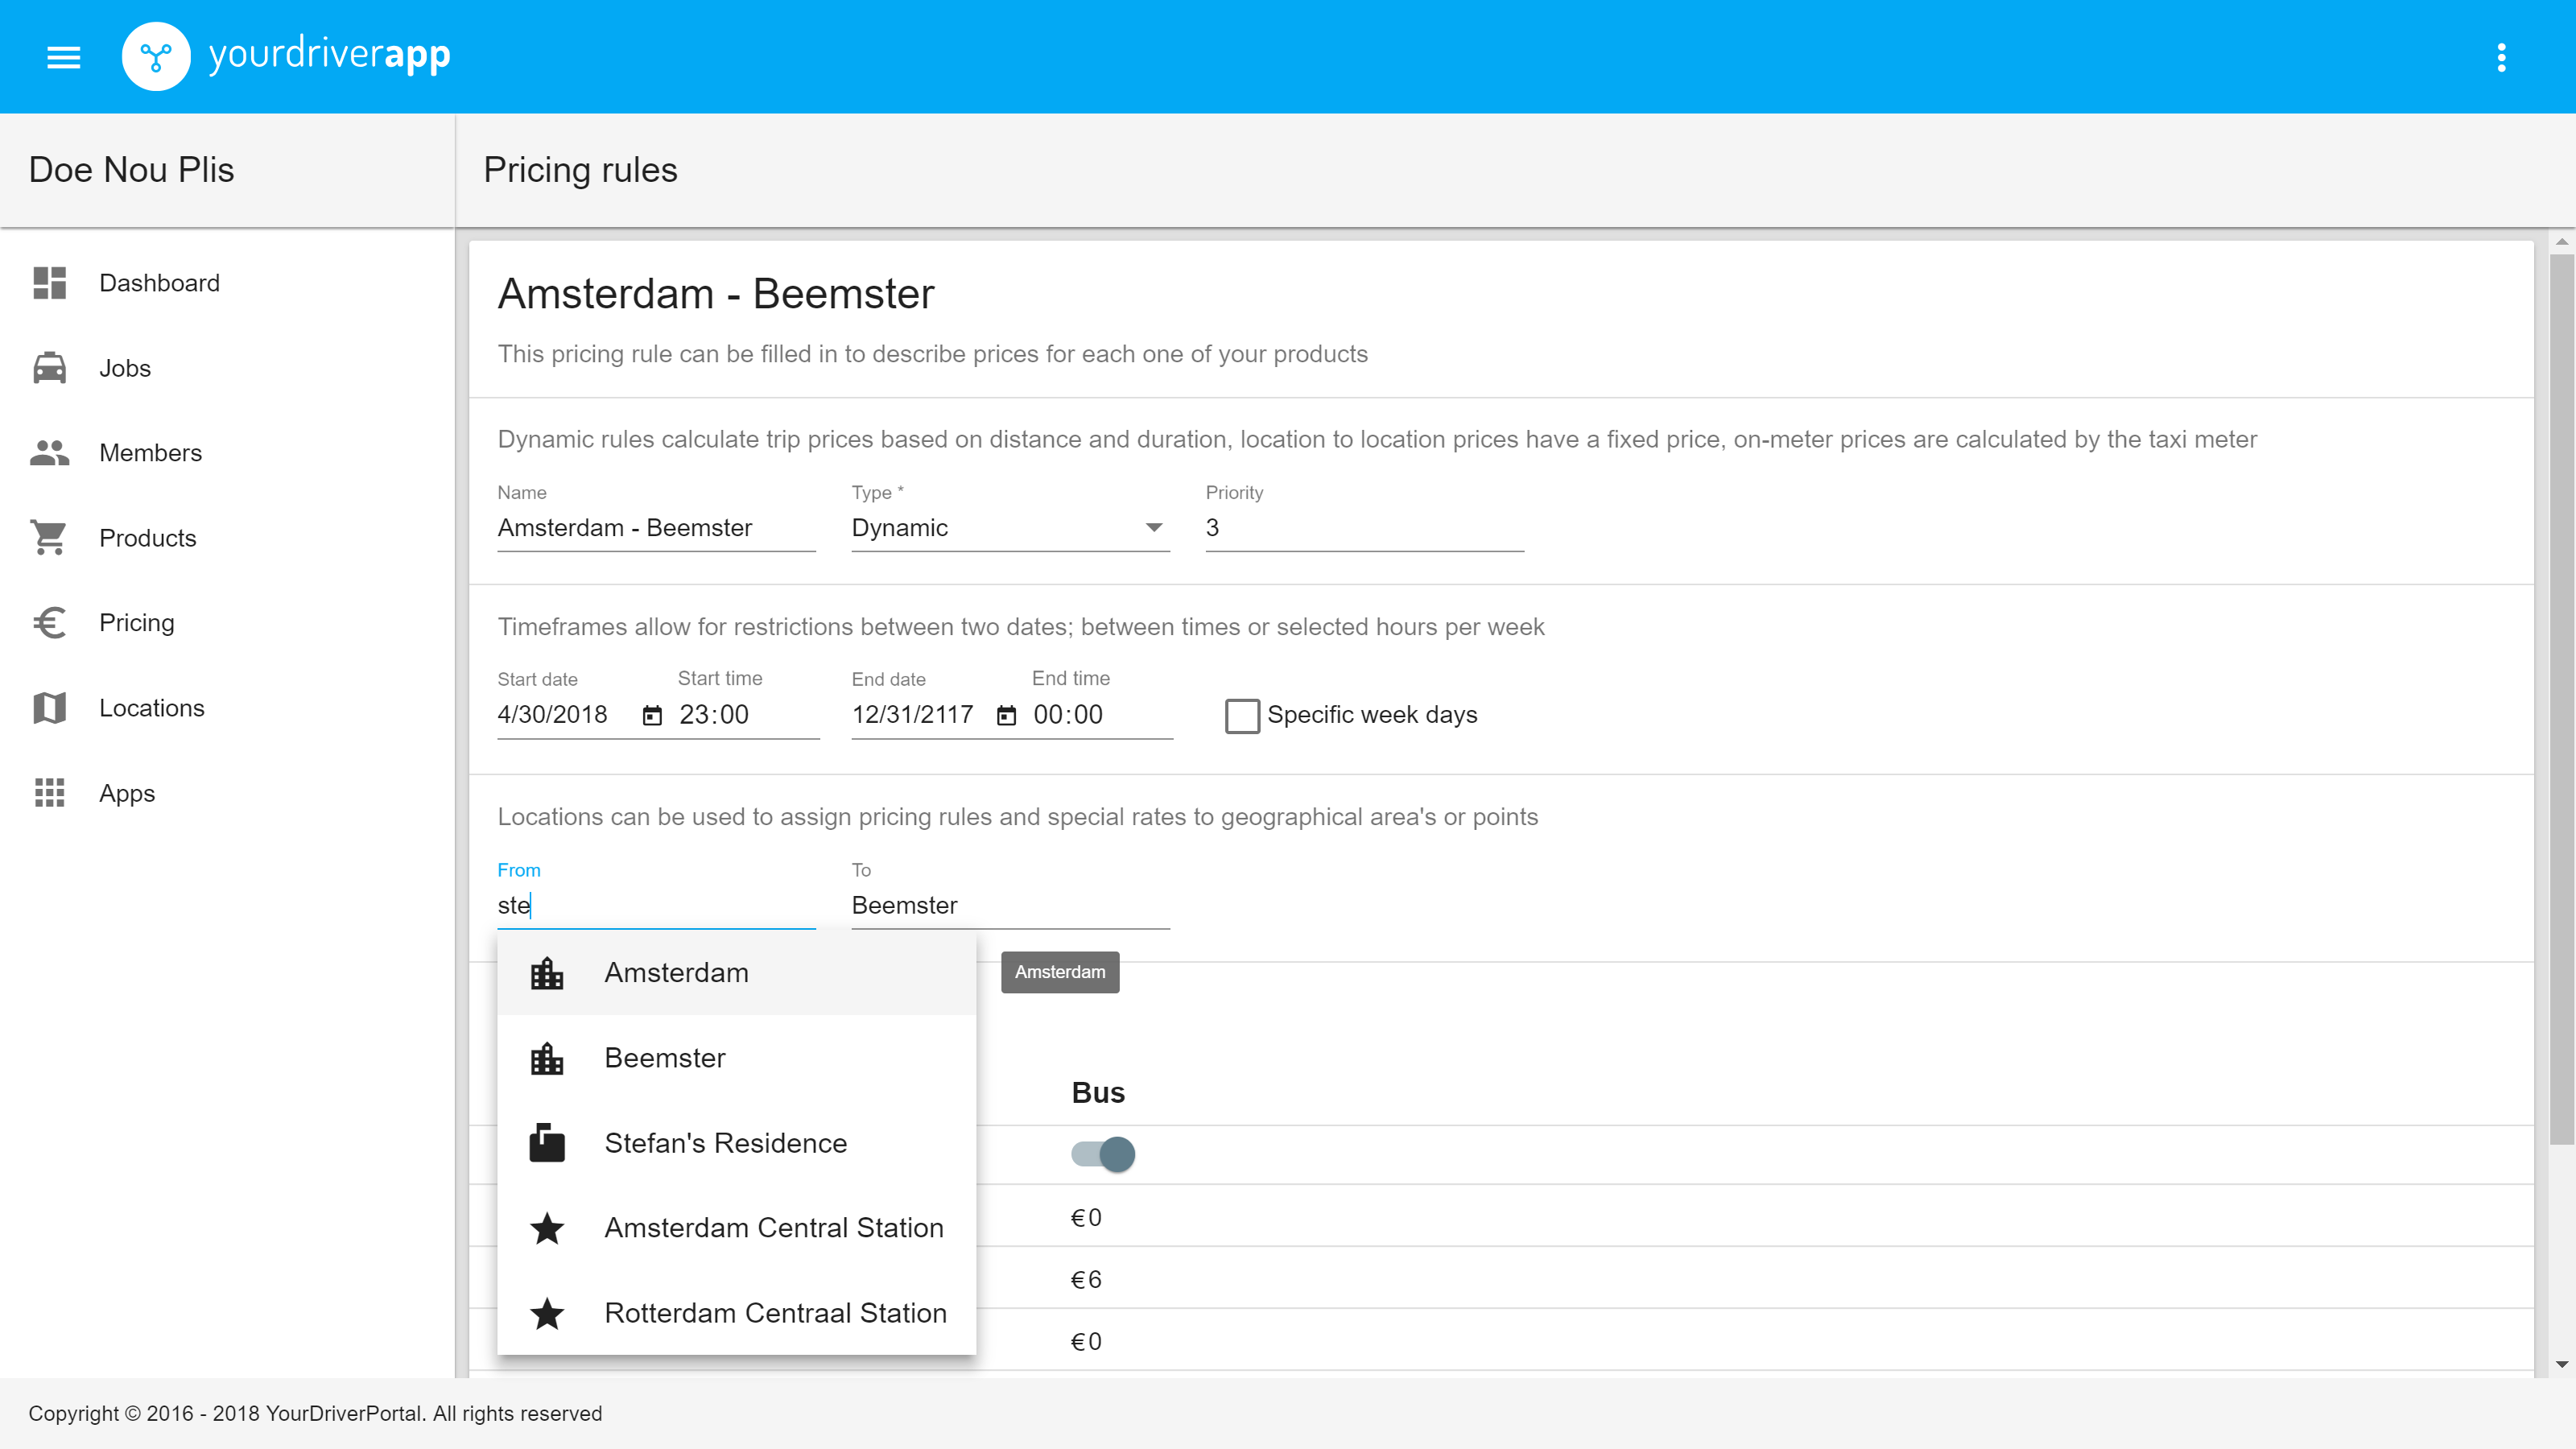
\includegraphics[width=0.9\textwidth]{Rules}
	\caption[Dynamic Form]{Dynamic Form.}
	\label{fig:Dynamic Form}
\end{figure}

The kilometer and minute price can be extended through thresholds. When a threshold is added, it copies the values from the row above, which may then be edited. A rule can be of type 'dynamic' and 'fixed', which transforms the form when changed. When the 'dynamic' type is selected, locations may be defined as 'Everywhere'. This is not the case for the 'fixed' type. This freedom would not make sense in most cases, therefore it is desired that a user defined a start and end location to avoid mistakes that have the potential of causing financial damage. The form only has the rows waiting price and fixed price, where the fixed price row holds the location inputs now. Because fixed prices can be extended with subrules like the kilometer and minute prices could be extended with thresholds, the locations have to be consistently associated with the fixed price.
%###############################################################################
% BEETJE OVER DESIGN
%###############################################################################

\subsection{Priority}
The priority for discounts and rules can be defined in the priority input field. For convenience, a drag and drop feature was added.
% #endregion

%%%%%%%%%%%%%%%%%%%%%%%%%%%%%%%%%%%%%%%%%%%%%%%%%%%%%%%%%%%%%%%%%%%%%%%%%%%%%%%%
% Locations
%%%%%%%%%%%%%%%%%%%%%%%%%%%%%%%%%%%%%%%%%%%%%%%%%%%%%%%%%%%%%%%%%%%%%%%%%%%%%%%%
% #region
\section{Locations}
Locations have been defined as either points or areas. In technical terms, this is sound. For an average user, this does not sound intuitive. That is why locations are named as two groups: locations and areas. The technical solution in matching points was initially based on points being distinct coordinate pairs, which could only be precisely matched if the user selected a location from the location service that was used, like Google Places. The locations found in searches would exactly match the coordinate pairs, as that is where the points are originated from. For practical purposes, a passenger may drop the pin on a map, which would have very little to no chance of matching the exact coordinate pair. That is why all locations are stored as polygons initially, with a coordinate pair denoting the centroid of the location. The polygons may be imported, drawn and edited by the user, depending on the location type.

%###############################################################################
% LOCATION SCREENSHOT
%###############################################################################
\begin{figure}[H]
	\centering
	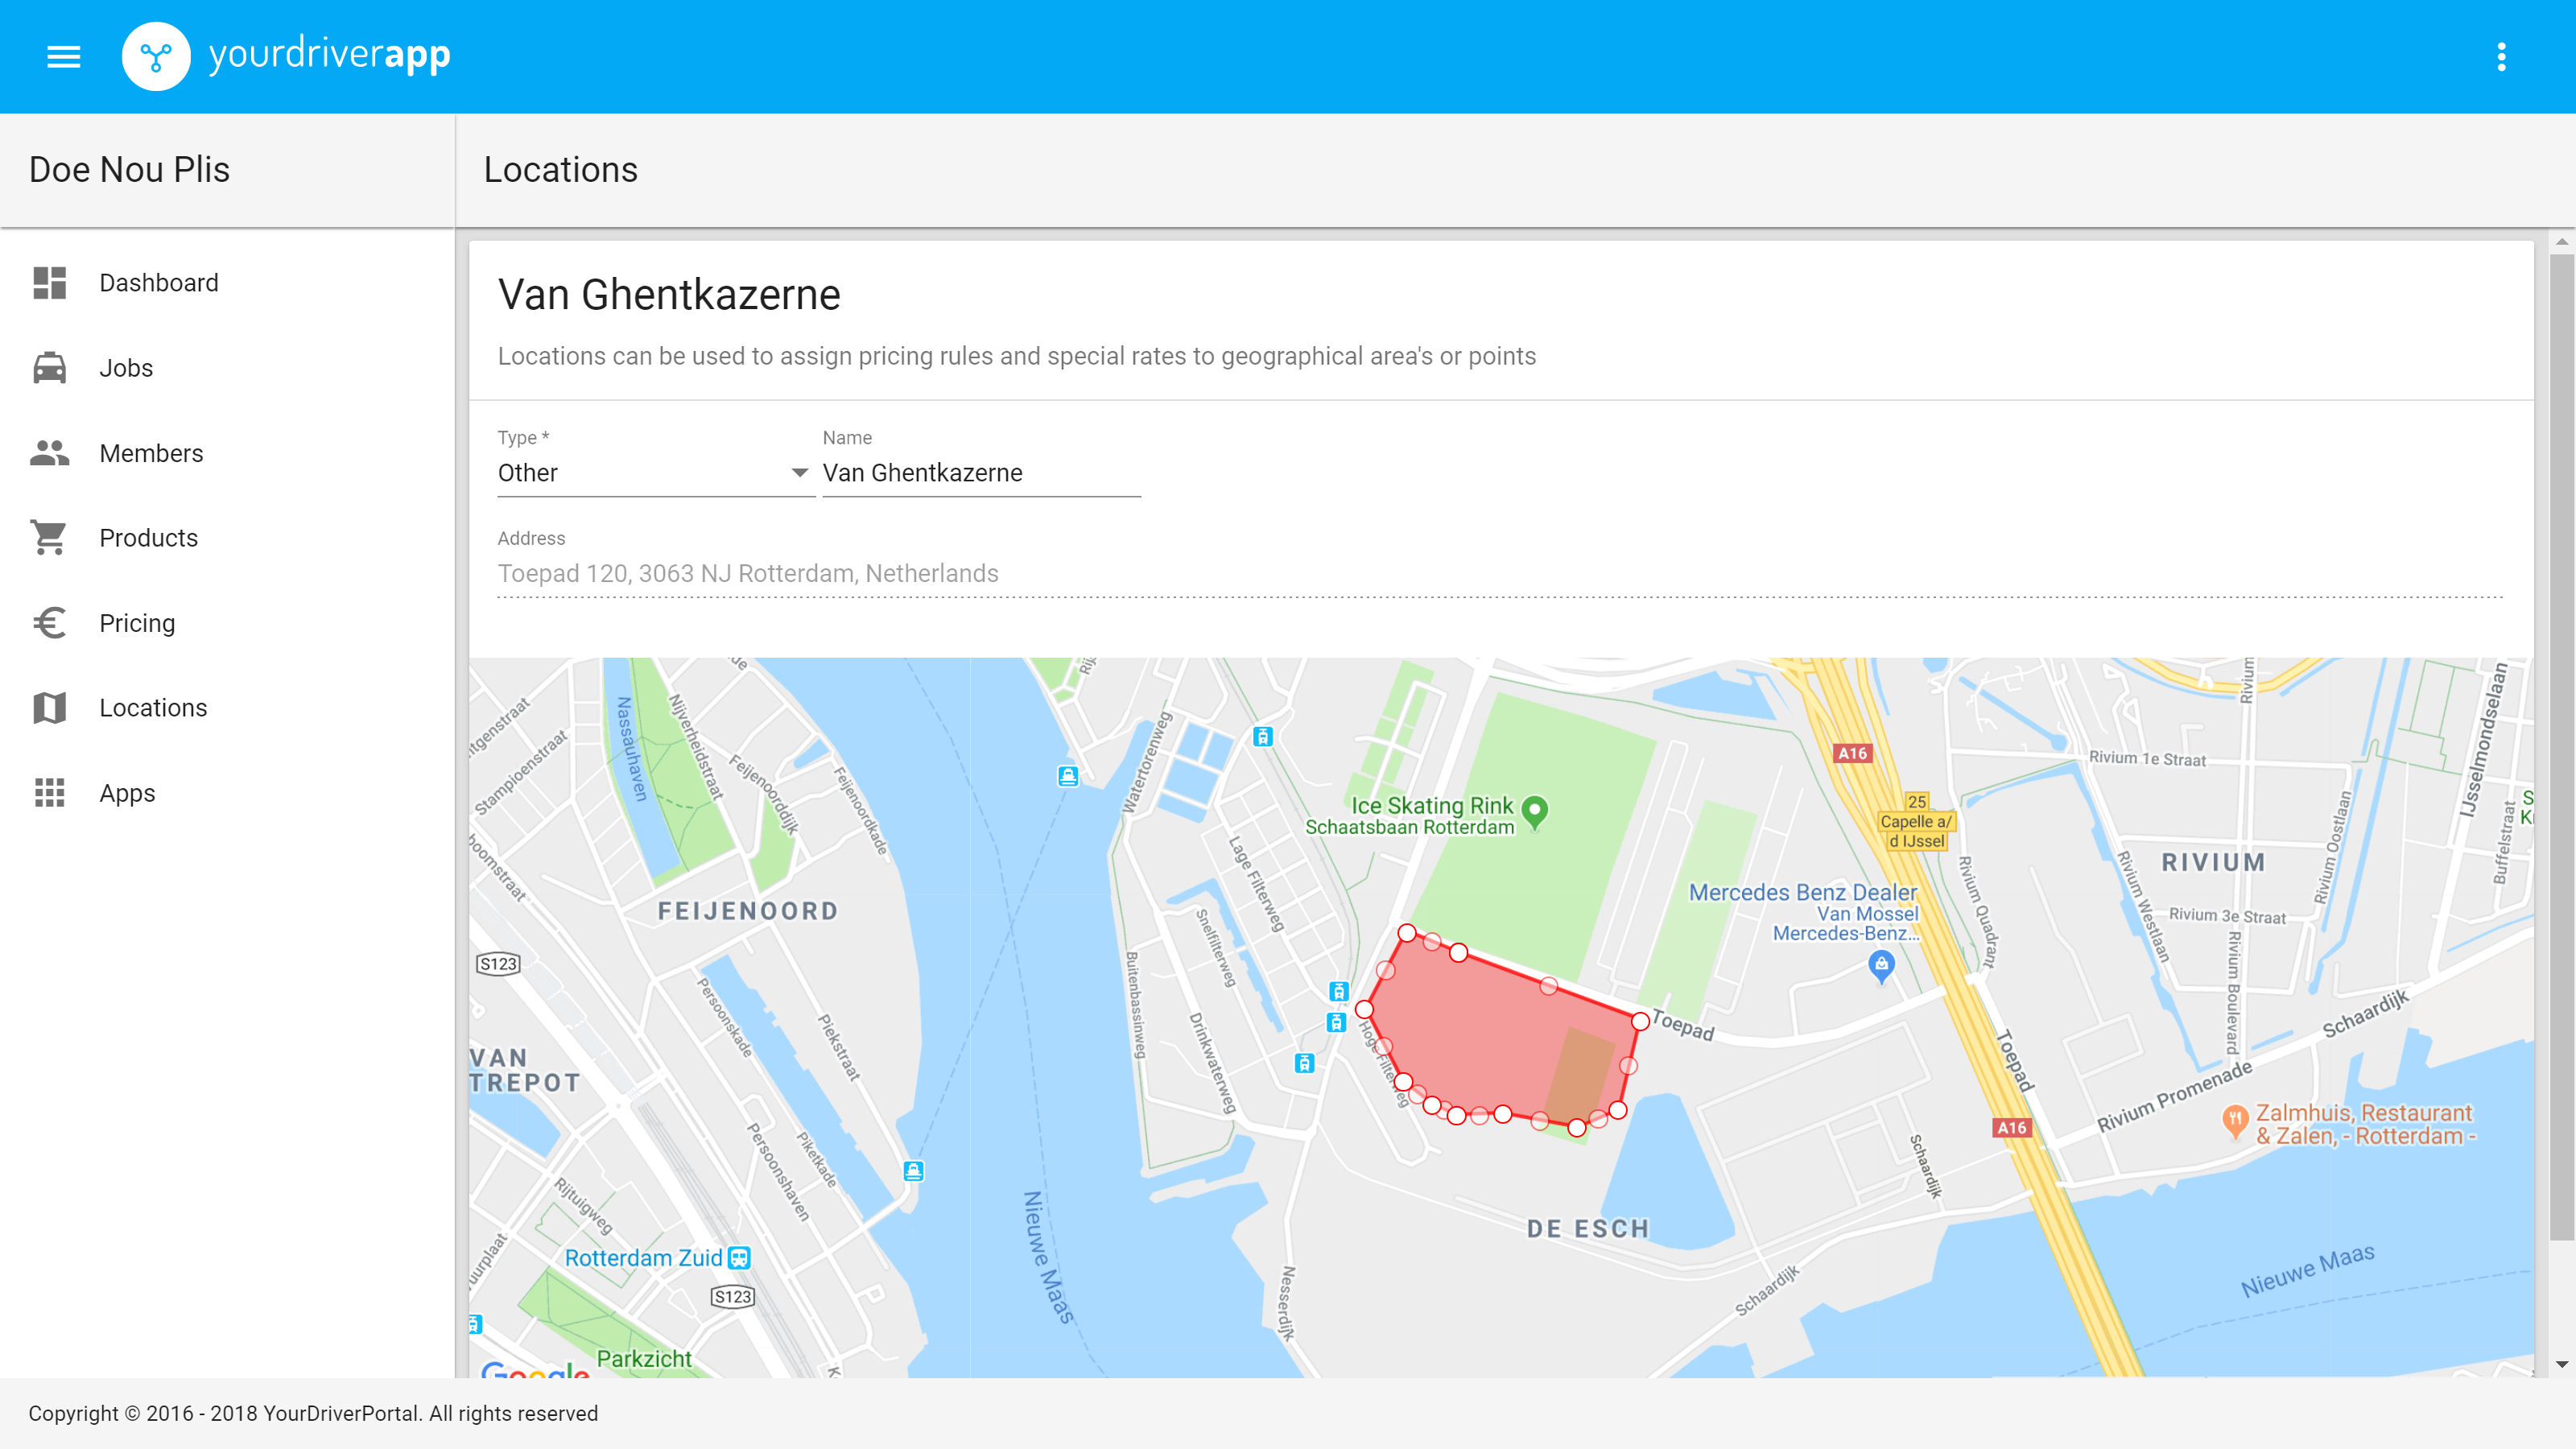
\includegraphics[width=0.9\textwidth]{Locations}
	\caption[Locations Overview]{Overview of points and areas.}
	\label{fig:Locations Overview}
\end{figure}

\subsection{Point}
When a point is created, only a search bar is visible initially. Autocomplete suggestions from Google Places are shown when the user starts typing. These results are filtered to only include addresses and smaller locations, to maintain the distinction between areas and points. A shape class has been created that is capable of plotting points, polygons and multipolygons on a Google Map using a method called autoDetect. When the user selects a location, the gps coordinates are used as a center around which a polygon is plotted.

\begin{center}
\noindent\begin{minipage}{.85\textwidth}
\begin{lstlisting}[caption={Generating Polygon From Point.}, label={lst:Generating Polygon From Point}]
/**
 * Generate a polygon around lat lng coordinates.
 */
private static fromPoint(
	lat: number,
	lng: number,
	theta: number,
	radius: number,
) {
	const points = [];
	const p = (lat, lng, x, y, r) =>
		[lat + (r * x), lng + (r * y) * 1.5];

	let x, y;
	let angle = 0.0;

	while (angle < 2 * Math.PI) {
		x = length * Math.cos(angle);
		y = length * Math.sin(angle);
		points.push(p(lat, lng, x, y, radius));
		angle += Math.abs(theta);
	}

	// Closing the polygon.
	points.push(points[0]);
	return Shape.fromPolygon(points);
}
\end{lstlisting}
\end{minipage}
\end{center}



- import

The distinction between points and areas is made in the sense that points are small locations a person could point at, like a house, hotel or a shop. Area's are bigger and more complex locations, like Schiphol or The Hague.

When a point is created, a user searches for a place in Google Places, gives it a name and a descriptor, and saves it as if it were a string of characters that would be matched within the system.

When an existing point is selected, the actual polygon is showing on the map.

\subsection{Area}
The area detail page contains
The map allows users to have more freedom in describing the location.

- import
- edit
-

When an area is created, the user has the freedom to start drawing on


% #endregion

%%%%%%%%%%%%%%%%%%%%%%%%%%%%%%%%%%%%%%%%%%%%%%%%%%%%%%%%%%%%%%%%%%%%%%%%%%%%%%%%
% Apps
%%%%%%%%%%%%%%%%%%%%%%%%%%%%%%%%%%%%%%%%%%%%%%%%%%%%%%%%%%%%%%%%%%%%%%%%%%%%%%%%
% #region
\section{Apps}
When a new rule or discount is saved, it is not activated by default. The app detail page allows rules and discounts to be associated with an application, upon which they become active. For pricing rules, the isFixed and isAllowedOnMeter settings may be set.

%###############################################################################
% APPS SCREENSHOT
%###############################################################################
\begin{figure}[H]
	\centering
	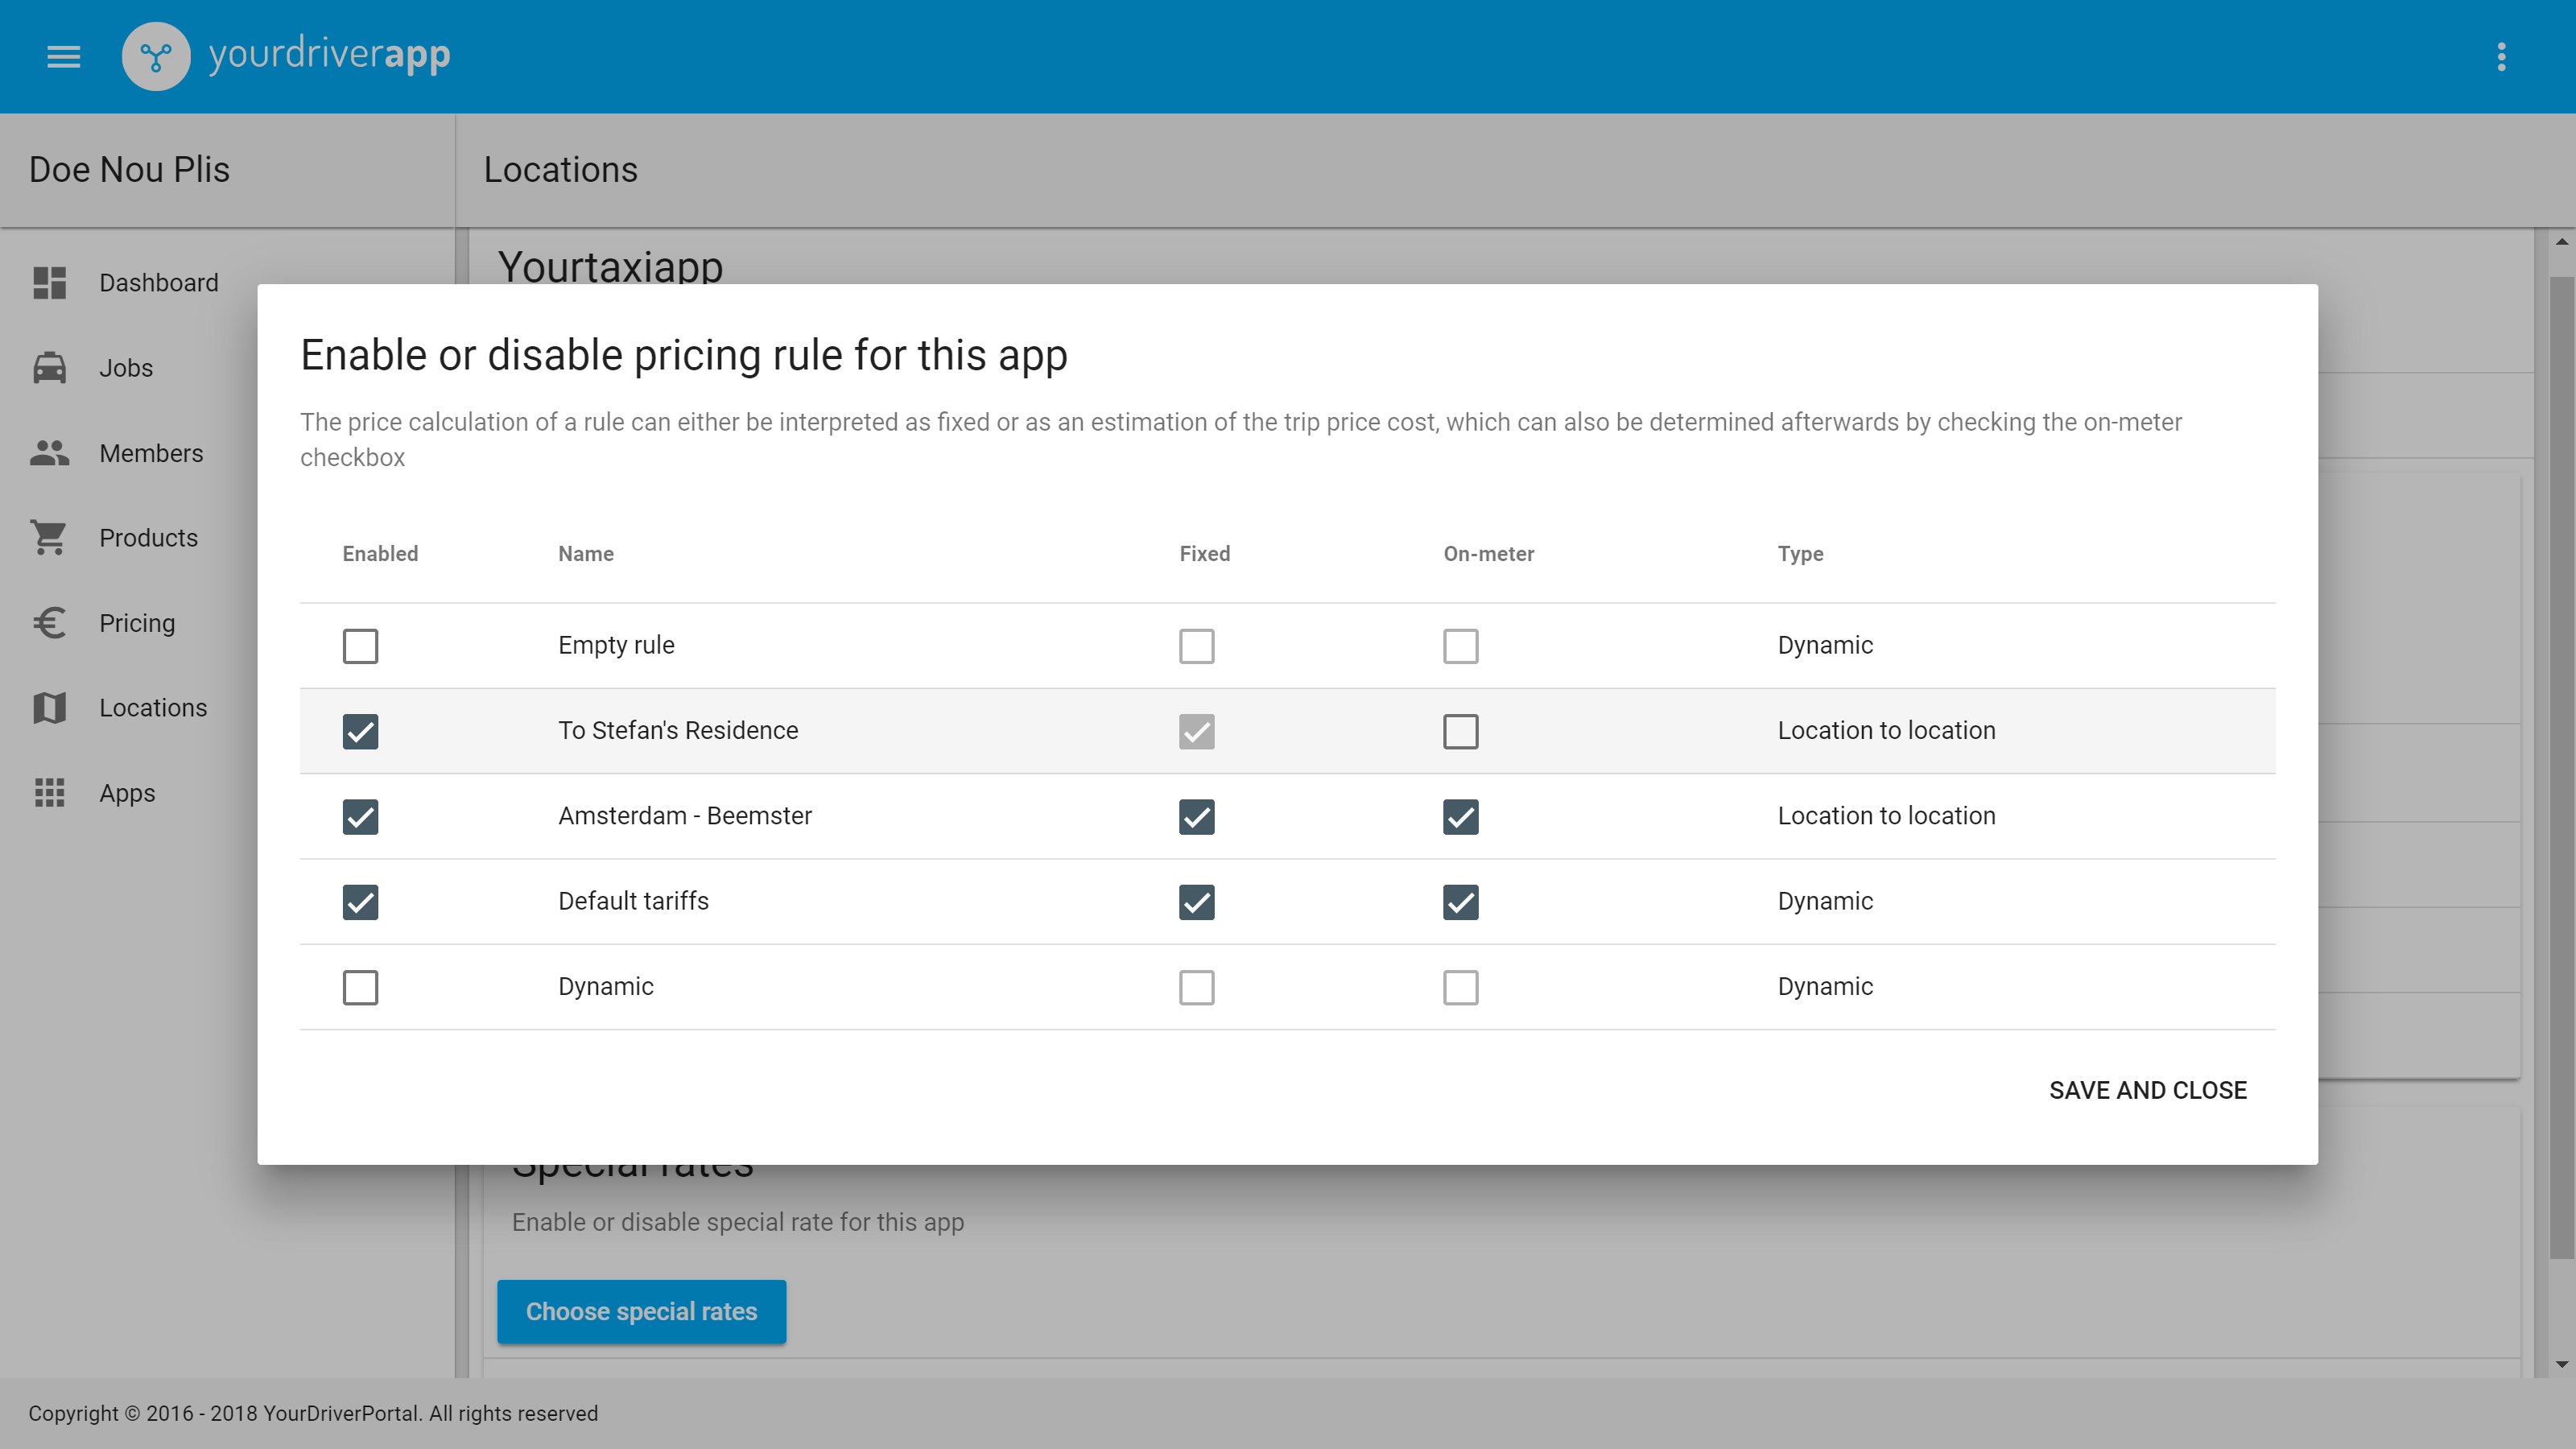
\includegraphics[width=0.9\textwidth]{Apps}
	\caption[Apps Detail Page]{Apps Detail Page.}
	\label{fig:Apps Detail Page}
\end{figure}

% #endregion

\section{Conclusion on The Portal}
\[\textit{Is it possible to communicate the inner workings of the system through the user interface?}\]\hfill

% Which backend concepts are essential to display in the frontend?
% Which design practices allow users to understand coherence of different elements that make up a rule?
% How should a user know what the outcome of his interactions with the system are?
